\newpage


\section{Model}

%%%%%%%%%%%%%%%%%%%%%%%%%%%%%%%%%%%%%%%%%%%%%%%%%%%%%%%%

\begin{comment}
task1:

基本参数设定:

假设温度为T(°C),时间t(天),光强l(cd),单个生菜最终鲜重m(g)

基本模型建立:

可以大致认为,光照强度和温度分别影响莴苣的生长,且二者不相互影响.设

\ref{e1}
\begin{equation}\label{e1}
	m=f(T)g(l)
\end{equation}

由常识可知:当T不变时,m在光饱和点之前随l增加而增加,当l达到光饱和点之后,m取值为定值;
当l不变时,m关于T先增后减(酶的活性与T有关).

故可假设$$g(l)=$$

$$f(T)=$$

模型求解:

根据所给数据拟合估计,求出$$g(l)=$$

$$f(T)=$$

由(1)

$$m=f(T)g(l)$$

task2:

基本参数设定:

设土地资源总量为S,单个个体吸收资源s_0,种植密度\rho(棵/m^2),c为工厂面积.

基本模型建立:

根据题意,种植密度只影响土地资源总量S的分配,也即m与个体吸收的土地资源总量呈正比.
在密度较小时,可以认为每个个体充分吸收所有土地资源;密度较大时,假设个体吸收相同的资源.

假设m与s_0呈线性关系$$m=h(s_0)=ks_0+b$$由h(0)=0得b=0.

显然
\ref{e1}
\begin{equation}\label{e1}
	S=cs_0\rho
\end{equation}

模型求解:

根据信息可知,s_0=时,m=500,故k=;

由此结合(2)得到m关于\rho的函数
\ref{e1}
\begin{equation}\label{e1}
	m=\frac{kS}{c\rho}
\end{equation}

task3:

基本参数设定:

设照明时间为t(h).工厂所需温度为$T_0$,外界温度为T,材料密度$\rho(n)$(kg·$m^{-3}$),热导率$\lambda(n)$(W·$m^{-2}$·$K^{-1}$),比热容c(n)(kJ·$kg^{-1}$·$K^{-1}$),总质量$m(n)=V\rho(n)$(V=)(n=1,2,3,4).工厂为长方体,令其水平长方形对角线与南北方向的纬线夹角为$\theta$作为朝向(两条对角线取小的那条).照明灯提供1cd光强所需功率为$p_0$(W·$h^{-1}$).总所需能量为E.注意由于题目考虑因素为温差,所以T的单位取°C或K不影响结果.

基本模型建立:

首先做一个基本假设,假设工厂先因其他条件到达一个温度,而后在不考虑其他影响下空调单独工作使温度到达$T_0$,所以空调消耗可视作以一天为一个单位.

在本题中,t=16.

空调负荷和温差成正比,可以认为
\begin{equation}\label{e1}
	Q=\left\{
\begin{aligned}
k(T-T_0) & , & T>T_0, \\
k(T_0-T) & , & T<T_0.
\end{aligned}
\right.
\end{equation}

$$W_1=\left\{
\begin{aligned}
2.5k(T-T_0) & , & T>T_0, \\
3.5k(T_0-T) & , & T<T_0.
\end{aligned}
\right.$$

灯照明功率为$W_2$,其中提供光强功率为$\frac{W_2}{2}$,散发热量$\frac{W_2}{2}$,

显然$$W_2=lp_0$$
\begin{equation}\label{e1}
	E=365W_1+365tW_2
\end{equation}

工厂体积V=,每立方米空气升高1°C所需热量$q_0=1.1921J$,那么在外界温度为$T_1$的情形时,在工厂内其他因素影响下工厂内温度
$$T=T_1+\frac{Q_{out}}{Vq_0}$$
$$Q_{out}=Q_{sun}+Q_{light}$$

太阳照射的有效面积为$S_{e}=h \cdot x \cdot cos\theta$,根据数据\ h=,x=.

太阳每天照射地球单位面积热量为$q_1=$,工厂表面积$S_{o}=$,墙面厚度\ y=,由此估算工厂外表面温度为
$$T_2=T_1+\frac{S_{e}q_1}{c(n)m(n)}$$
$$Q_{sun}={\lambda}(n)\frac{(T_2-T)S_{o}}{y}$$
$$Q_{light}=t\frac{W_2}{2}$$

task4:

基本参数设定:

设照明时间为t(h),则得到新的m的函数$$m=f(T)g(l,t)$$

基本模型建立:

为平衡产量和能源消耗,认为二者权重一样,在task3中使t=24求出$Q_{max}$,取$m_{max}=500$

定义目标函数
\begin{equation}\label{e1}
	\omega=\frac{m}{m_{max}}-\frac{Q}{Q_{max}}
\end{equation}
求出$\omega_{max}$=,此时各项变量为

\end{comment}

%%%%%%%%%%%%%%%%%%%%%%%%%%%%%%%%%%%%%%%%%%%%%%%%%%%%%%%%%%%%%%%%%%%
\subsection{Model I}

\begin{comment}
为了满足任务一的要求,我们建立了模型一,模型具体的内容已在第二章详细说明。这里阐述一下模型的设置思路与方法。
\end{comment}

In order to meet the requirements of Task 1, we set up Model 1, the details of which have been described in detail in Chapter 2. The ideas and methods of model setup are described here.
\\

\textbf{Basic Parameter Setting for Model I:}

Assuming the temperature is T (°C), time t (days), light intensity l (cd), individual lettuce final fresh weight m (g)
\\

\textbf{Basic Model Building for Model I:}


It can be roughly concluded that light intensity and temperature affect the growth of lettuce respectively, and the two do not affect each other. Establish

%\ref{e1}
\begin{equation}\label{e1}
	m=f(T)g(l)
\end{equation}

It can be known from common sense: when T is unchanged, m increases with the increase of l before the light saturation point, and when l reaches the light saturation point, the value of m is fixed;
When l does not change, \textit{m} increases and then decreases with respect to T (enzyme activity is related to T).\\
Our reference data is shown below.
\begin{figure}[h]
    \centering
    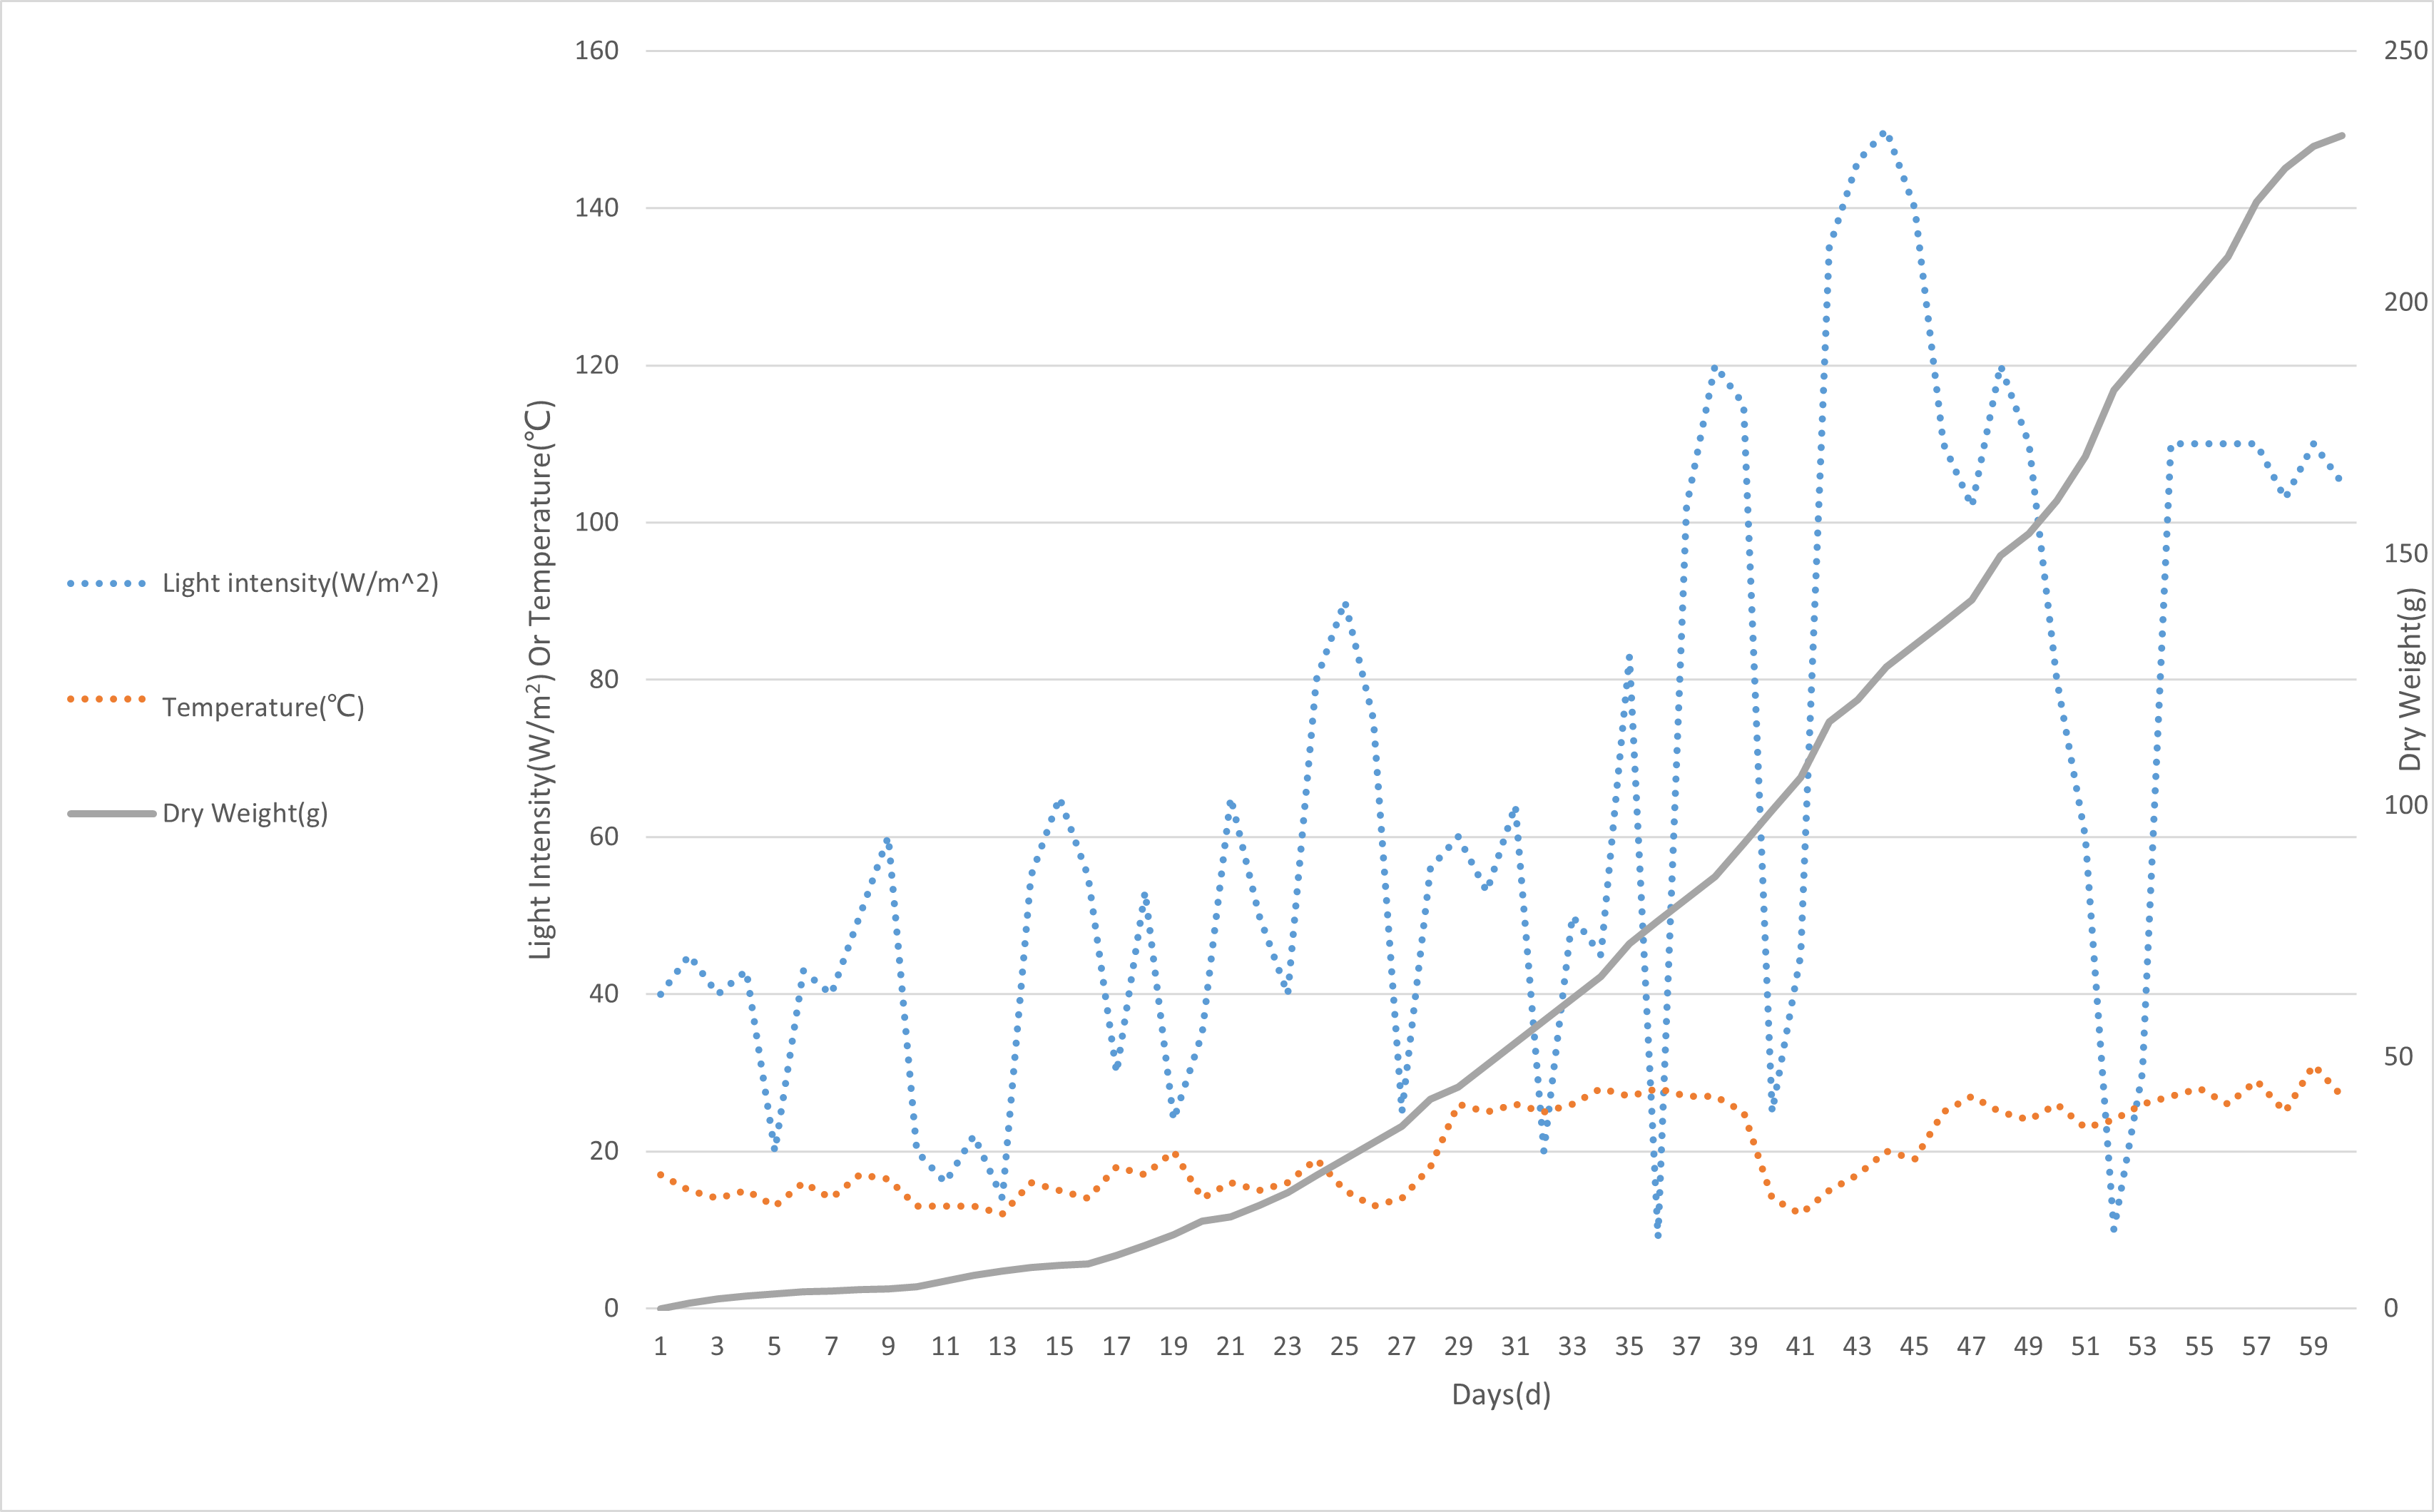
\includegraphics[scale=0.5]{{figure/Model I Data.png}}%插入图片的指令
    \caption{The Growth Trend of a Lettuce in 60 Days in Different Light Intensity and Temperature}%标题
    \label{Label}
\end{figure}


Looking at our data graphs, we can see that the temperature formulas are in a quadratic polynomial relationship, while the light intensity formulas are in an exponential relationship therefore we make the following assumptions.
\begin{equation}\label{e1}
	m=f(T)g(l)
\end{equation}

\begin{equation}\label{e1}
	g(l)=  a_1+b_1e^{c_1(l+d_1)}
\end{equation}
\begin{equation}\label{e1}
	f(T)= a_2\mathop{{T}}\nolimits^{{2}}+b_2T+c_2 
\end{equation}

Where \textit{a,b,c,d }are all parameters.
\\
\\
\newpage


\textbf{Model Solving for Task 1:}

Based on the given data, the estimation is fitted
\begin{equation}\label{e1}
	g(l)= 10.702-6.937e^{-\frac{l-0.22}{4.02}}
\end{equation}

\begin{equation}\label{e1}
	f(T)= -0.0009\mathop{{T}}\nolimits^{{2}} + 0.3171T + 11.091
\end{equation}
 \label{el}

from(1)


\begin{equation}\label{e1}
	m=f(T)g(l)= (10.702-6.937e^{-\frac{l-0.22}{4.02}})(-0.0009\mathop{{T}}\nolimits^{{2}} + 0.3171T + 11.091)
\end{equation}

We performed data validation with the model and the results are as follows.

\begin{figure}[h]
    \centering
    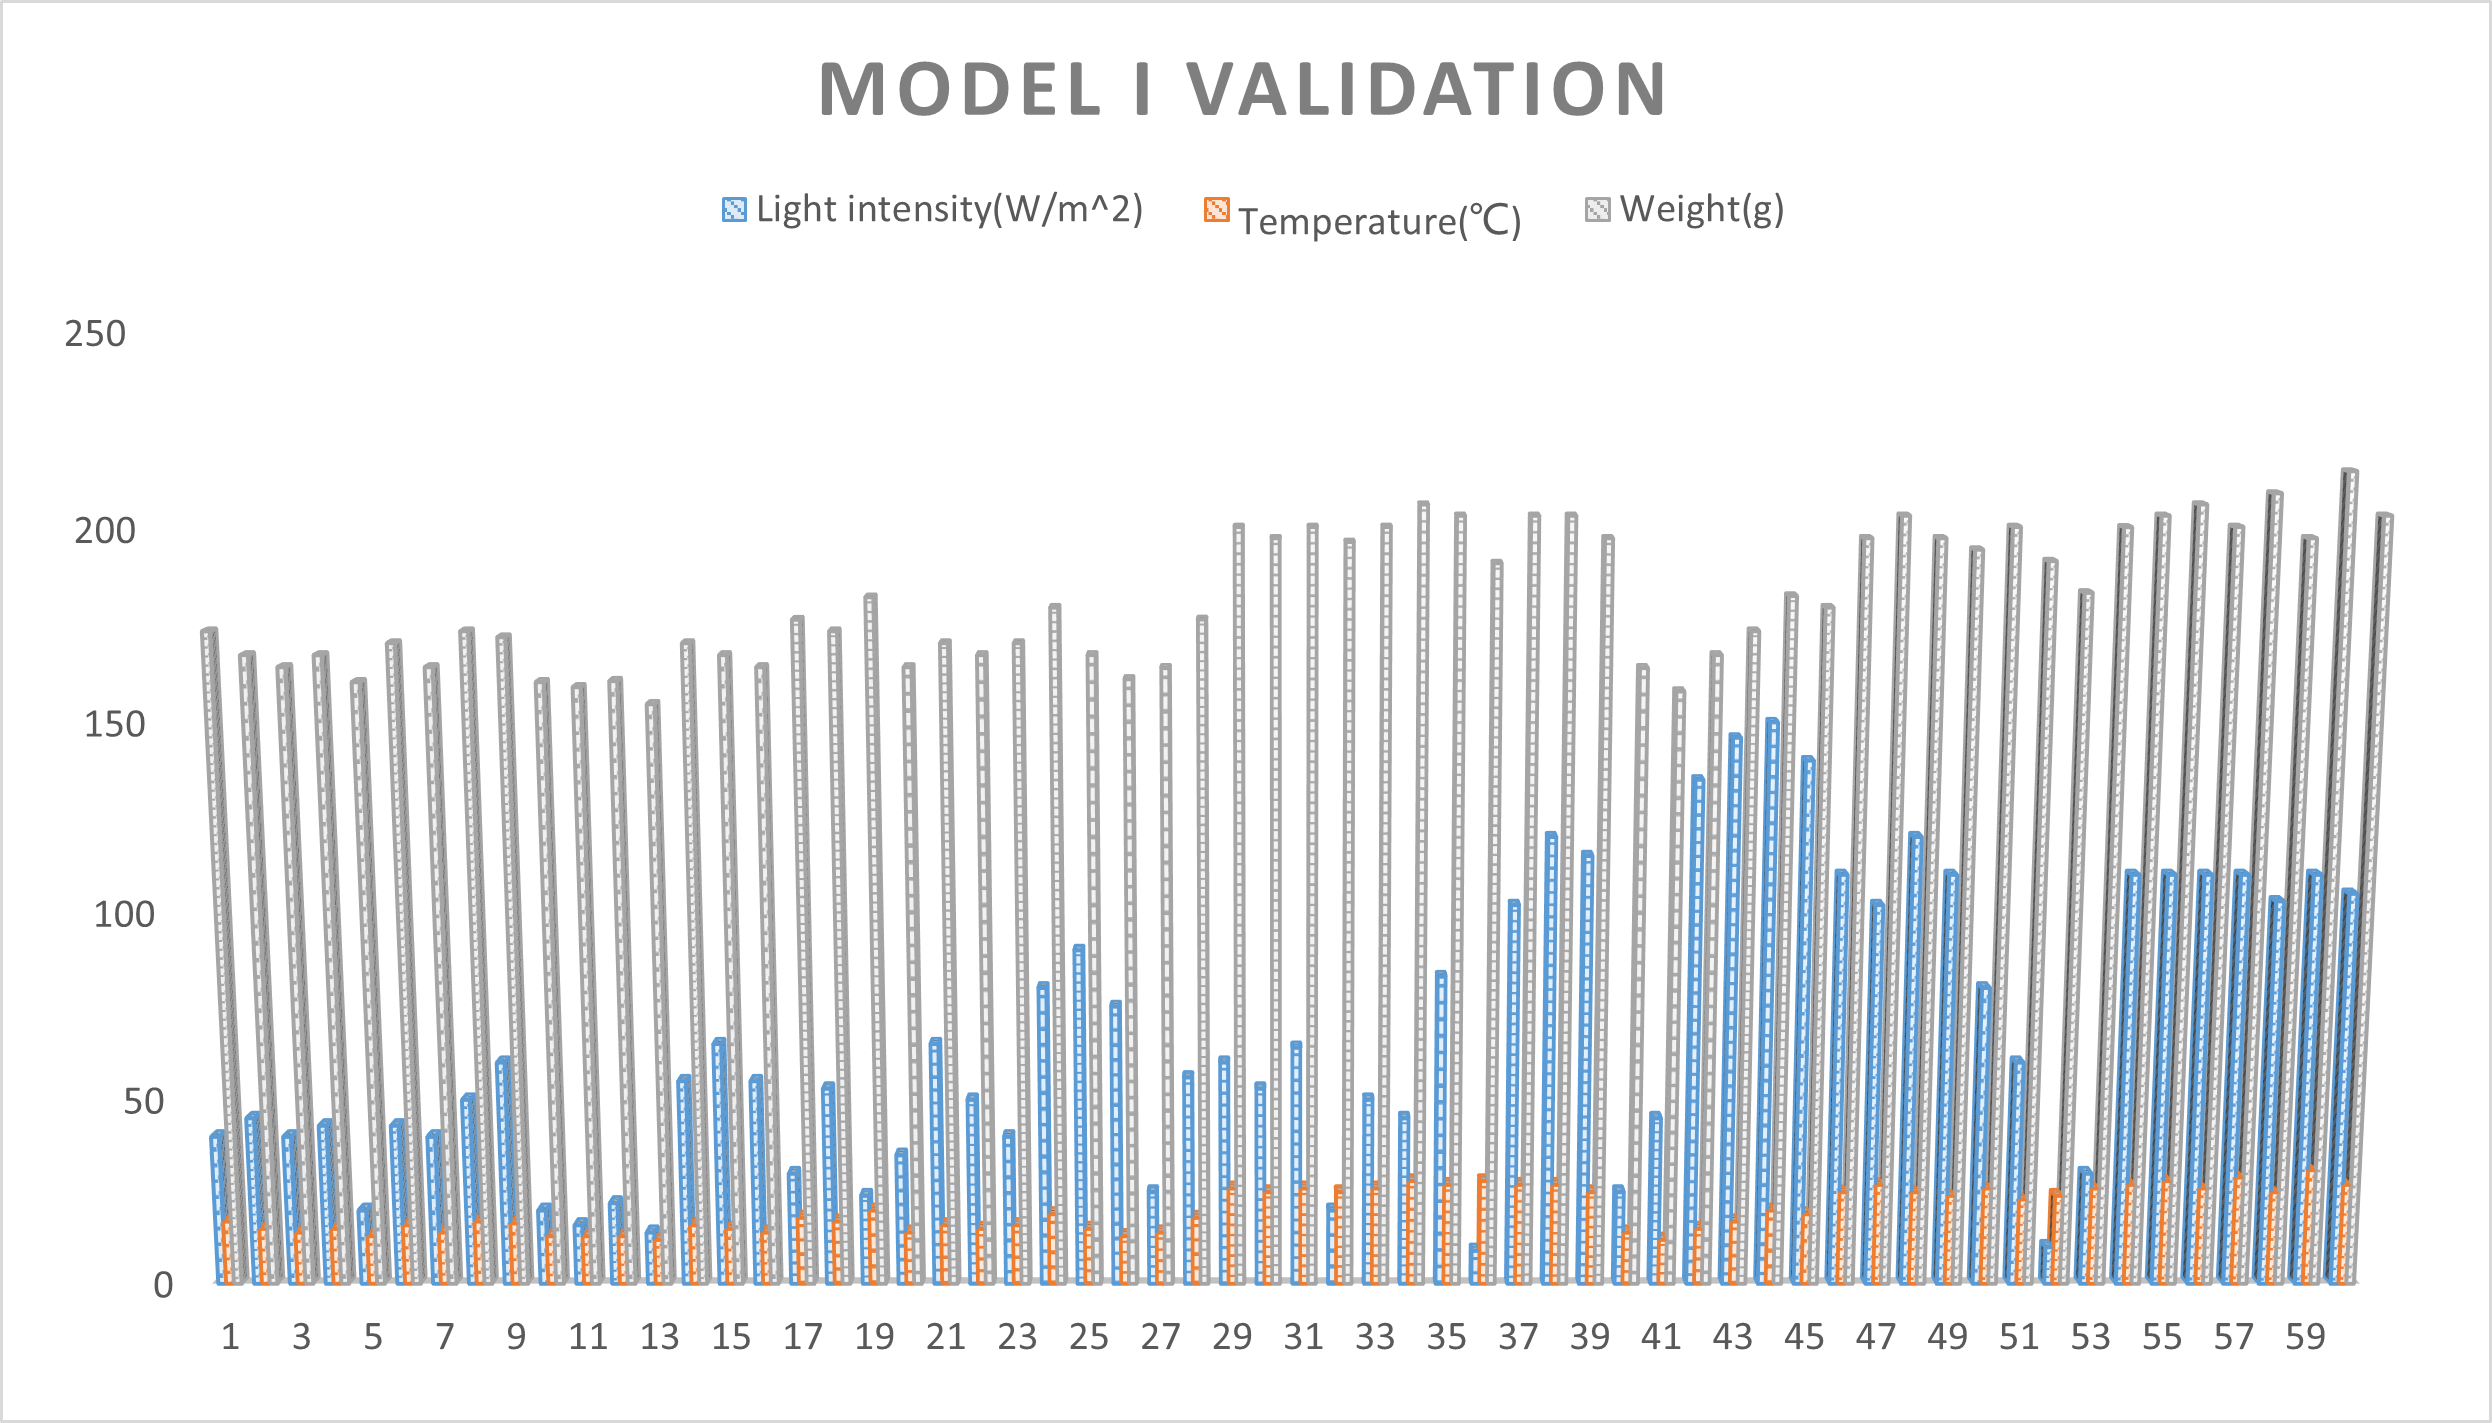
\includegraphics[scale=0.7]{{figure/Model I Vadiation.png}}%插入图片的指令
    \caption{Model I Validation}%标题
    \label{Label}
\end{figure}

We found that most of the vegetables were concentrated between 150g and 200g, which is in good agreement with the facts. Also the model can be helpful for Task 2.
%%%%%%%%%%%%%%%%%%%%%%%%%%%%%%%%%%%%%%%%%%%%%%%%%
\newpage
\subsection{Model II}
\begin{comment}
对于任务二,我们建立模型二。基本设置如下。
\end{comment}

For Task 2, we build Model 2. The basic setup is as follows\\

\textbf{Basic Parameter Setting for Model II:}

Let the total amount of land resources be S, the $s_0$\ of resources absorbed by a single individual, the planting density $\rho$(tree/$m^2$), and\ c\ be\ the area\ of\ the\ factory.\\

\textbf{Basic Model Building for Model II:}

According to the title, planting density only affects the distribution of total land resources S, that is, m is proportional to the total amount of land resources absorbed by individuals.
At low densities, it can be considered that each individual fully absorbs all land resources; When the density is large, it is assumed that individuals absorb the same resources.

Suppose m has a linear relationship with $s_0$:
\begin{equation}\label{e1}
	m=h(s_0)=ks_0+b 
\end{equation}


From\ h(0)=0 to b=0.

Apparently,
%\ref{e1}
\begin{equation}\label{e1}
	S=cs_0\rho
\end{equation}
\\

\textbf{Model Solving for Task 2:}

According to the information, when $s_0$=103, m=500, c=14.884, so k≈4.85;

This combines (2) to obtain the function of m with respect to $\rho$
%\ref{e1}
\begin{equation}\label{e1}
	m=\frac{kS}{c\rho}=\frac{4.85S}{14.884\rho}≈0.326\frac{S}{\rho}
\end{equation}
\\
We next used the model to make predictions.We assume that the number of lettuce per unit area is 3. Based on the container size of 20 feet, we predict the following results.

\begin{figure}[h]
    \centering
    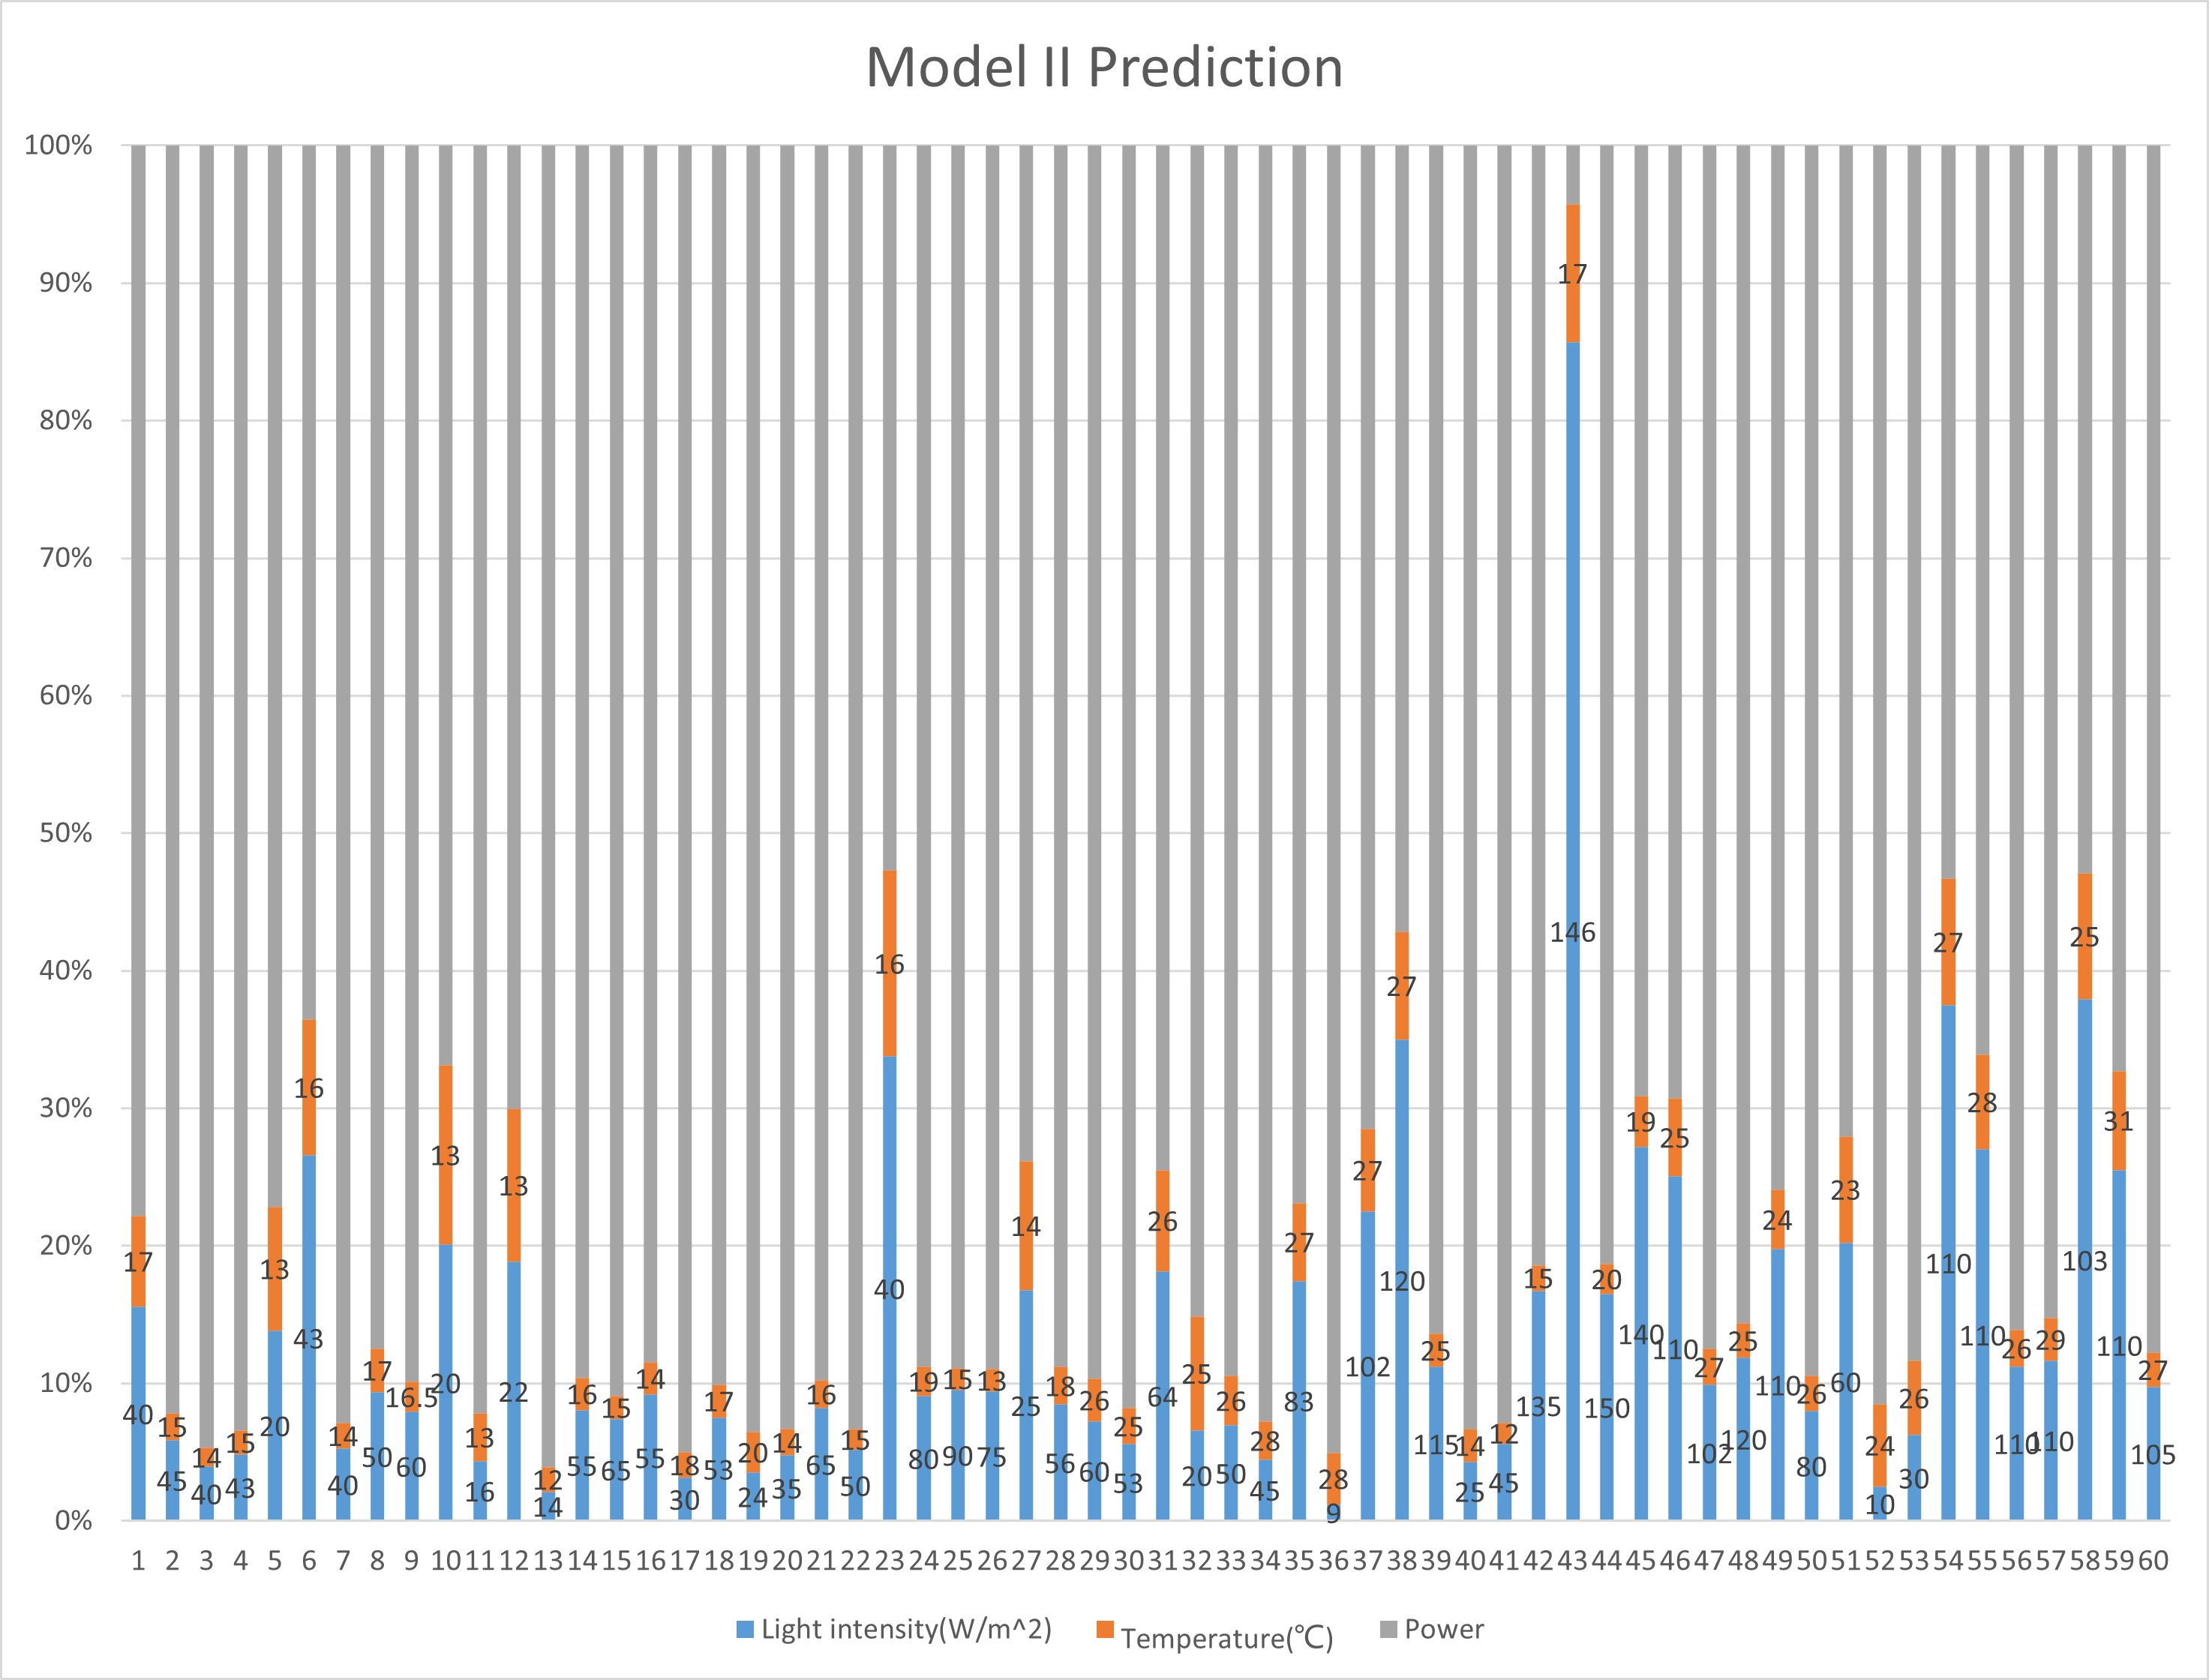
\includegraphics[scale=0.7]{{figure/Model II Prediction.png}}%插入图片的指令
    \caption{Model II Prediction for Random Light Intensity }%标题
    \label{Label}
\end{figure}

We predicted Model II with random light intensity and temperature, and the prediction results were more consistent with the relevant data we obtained, within 10 percent error, with a high degree of confidence.


\subsection{Model III}

\textbf{Basic Parameter Setting for Model III:}


The required temperature of the plant is $T_0$, the outside temperature is T, the material density is $\rho(n)$(kg·$m^{-3}$), thermal conductivity $\lambda(n)$(W·$m^{-2}$·$K^{-1}$), specific heat capacity c(n)(kJ·$kg^{-1}$·$K^{-1}$), total mass $m(n)=V\rho(n)$($V=s_1\cdot\lambda(n)$, $s_1$ is the surface area of the container, and n=1,2,3,4). Let its horizontal rectangular diagonal and the latitude line in the north-south direction be $\theta$ as the orientation (the smaller of the two diagonals).The power required for the lamp to provide 1cd light intensity is $p_0$(W·$h^{-1}$).The total required energy is E. Note that since the topic consideration factor is the temperature difference, the unit of T takes °C or K does not affect the result.\\

\\
\\ \hspace*{\fill} \\

\textbf{Basic Model Building for Model III:}


First of all, make a basic assumption, suppose that the factory first reaches a temperature due to other conditions, and then the air conditioner works alone to make the temperature reach $T_0$ without considering other influences, so the air conditioning consumption can be regarded as a unit of a day.

The air conditioning load is proportional to the temperature difference, it can be considered
\begin{equation}\label{e1}
	Q=\left\{
\begin{aligned}\label{el}
k(T-T_0) & , & T>T_0, \\
k(T_0-T) & , & T<T_0.
\end{aligned}
\right.
\end{equation}
\begin{equation}\label{e1}
W_1=\left\{
\begin{aligned}
2.5k(T-T_0) & , & T>T_0, \\
3.5k(T_0-T) & , & T<T_0.
\end{aligned}
\right.
\end{equation}


The lamp lighting power is $W_2$, where the light intensity power provided is $\frac{W_2}{2}$, and the heat dissipated $\frac{W_2}{2}$,

Apparently 
\begin{equation}\label{e1}
	W_2=lp_0
\end{equation}

\begin{equation}\label{e1}
	E=365W_1+16 \times 365W_2
\end{equation}


Factory volume $V_0$=39.14$m^3$,the heat required to increase 1 °C per cubic meter of air is $q_0=1.1921J$, so when the outside temperature is $T_1$, the temperature in the factory is affected by other factors in the factory
\begin{equation}\label{e1}
	T=T_1+\frac{Q_{out}}{V_0q_0}
\end{equation}

\begin{equation}\label{e1}
	Q_{out}=Q_{sun}+Q_{light}
\end{equation}


The effective area of solar irradiation is $S_{e}=h \cdot x \cdot cos\theta$, according to the data  h=2.63m,x=6.10m.

The heat per unit area of the sun hitting the earth is $q_1=1367J$ per second, the factory surface area is $S_{o}=58.64m^2$, and the wall thickness  $y=2.2mm$, from which the temperature of the outer surface of the factory is estimated
\begin{equation}\label{e1}
	T_2=T_1+\frac{S_{e}q_1}{c(n)m(n)}
\end{equation}


\begin{equation}\label{e1}
	Q_{sun}={\lambda}(n)\frac{(T_2-T)S_{o}}{y}
\end{equation}

\begin{equation}\label{e1}
	Q_{light}=16 \times \frac{W_2}{2}=8{W_2}
\end{equation}


%%%%%%%%%%%%%%%%%%%%%%%%%%%%%%%%%%%%%%%%%%%%%%

\subsection{Application 1: Fresh weight energy model for lettuce}

Tasks 4 requires us to calculate the overall energy consumption separately. We performed separate analytical estimates using the models described above. The analysis process is as follows.


Basic parameter setting:

If the illumination time is t(h), we get the new function of m
\begin{equation}\label{e1}
	m=f(T)g(l,t)
\end{equation}


Basic model building:

In order to balance the yield and energy consumption, considering that the weights of the two are the same, let t=24 find $Q_{max}$ in task3, and take $m_{max}=500$

Define the objective function
\begin{equation}\label{e1}
	\omega=\frac{m}{m_{max}}-\frac{Q}{Q_{max}}
\end{equation}

Find $\omega_{max}$=307, which satisfies our needs above.

\begin{figure}[h]
    \centering
    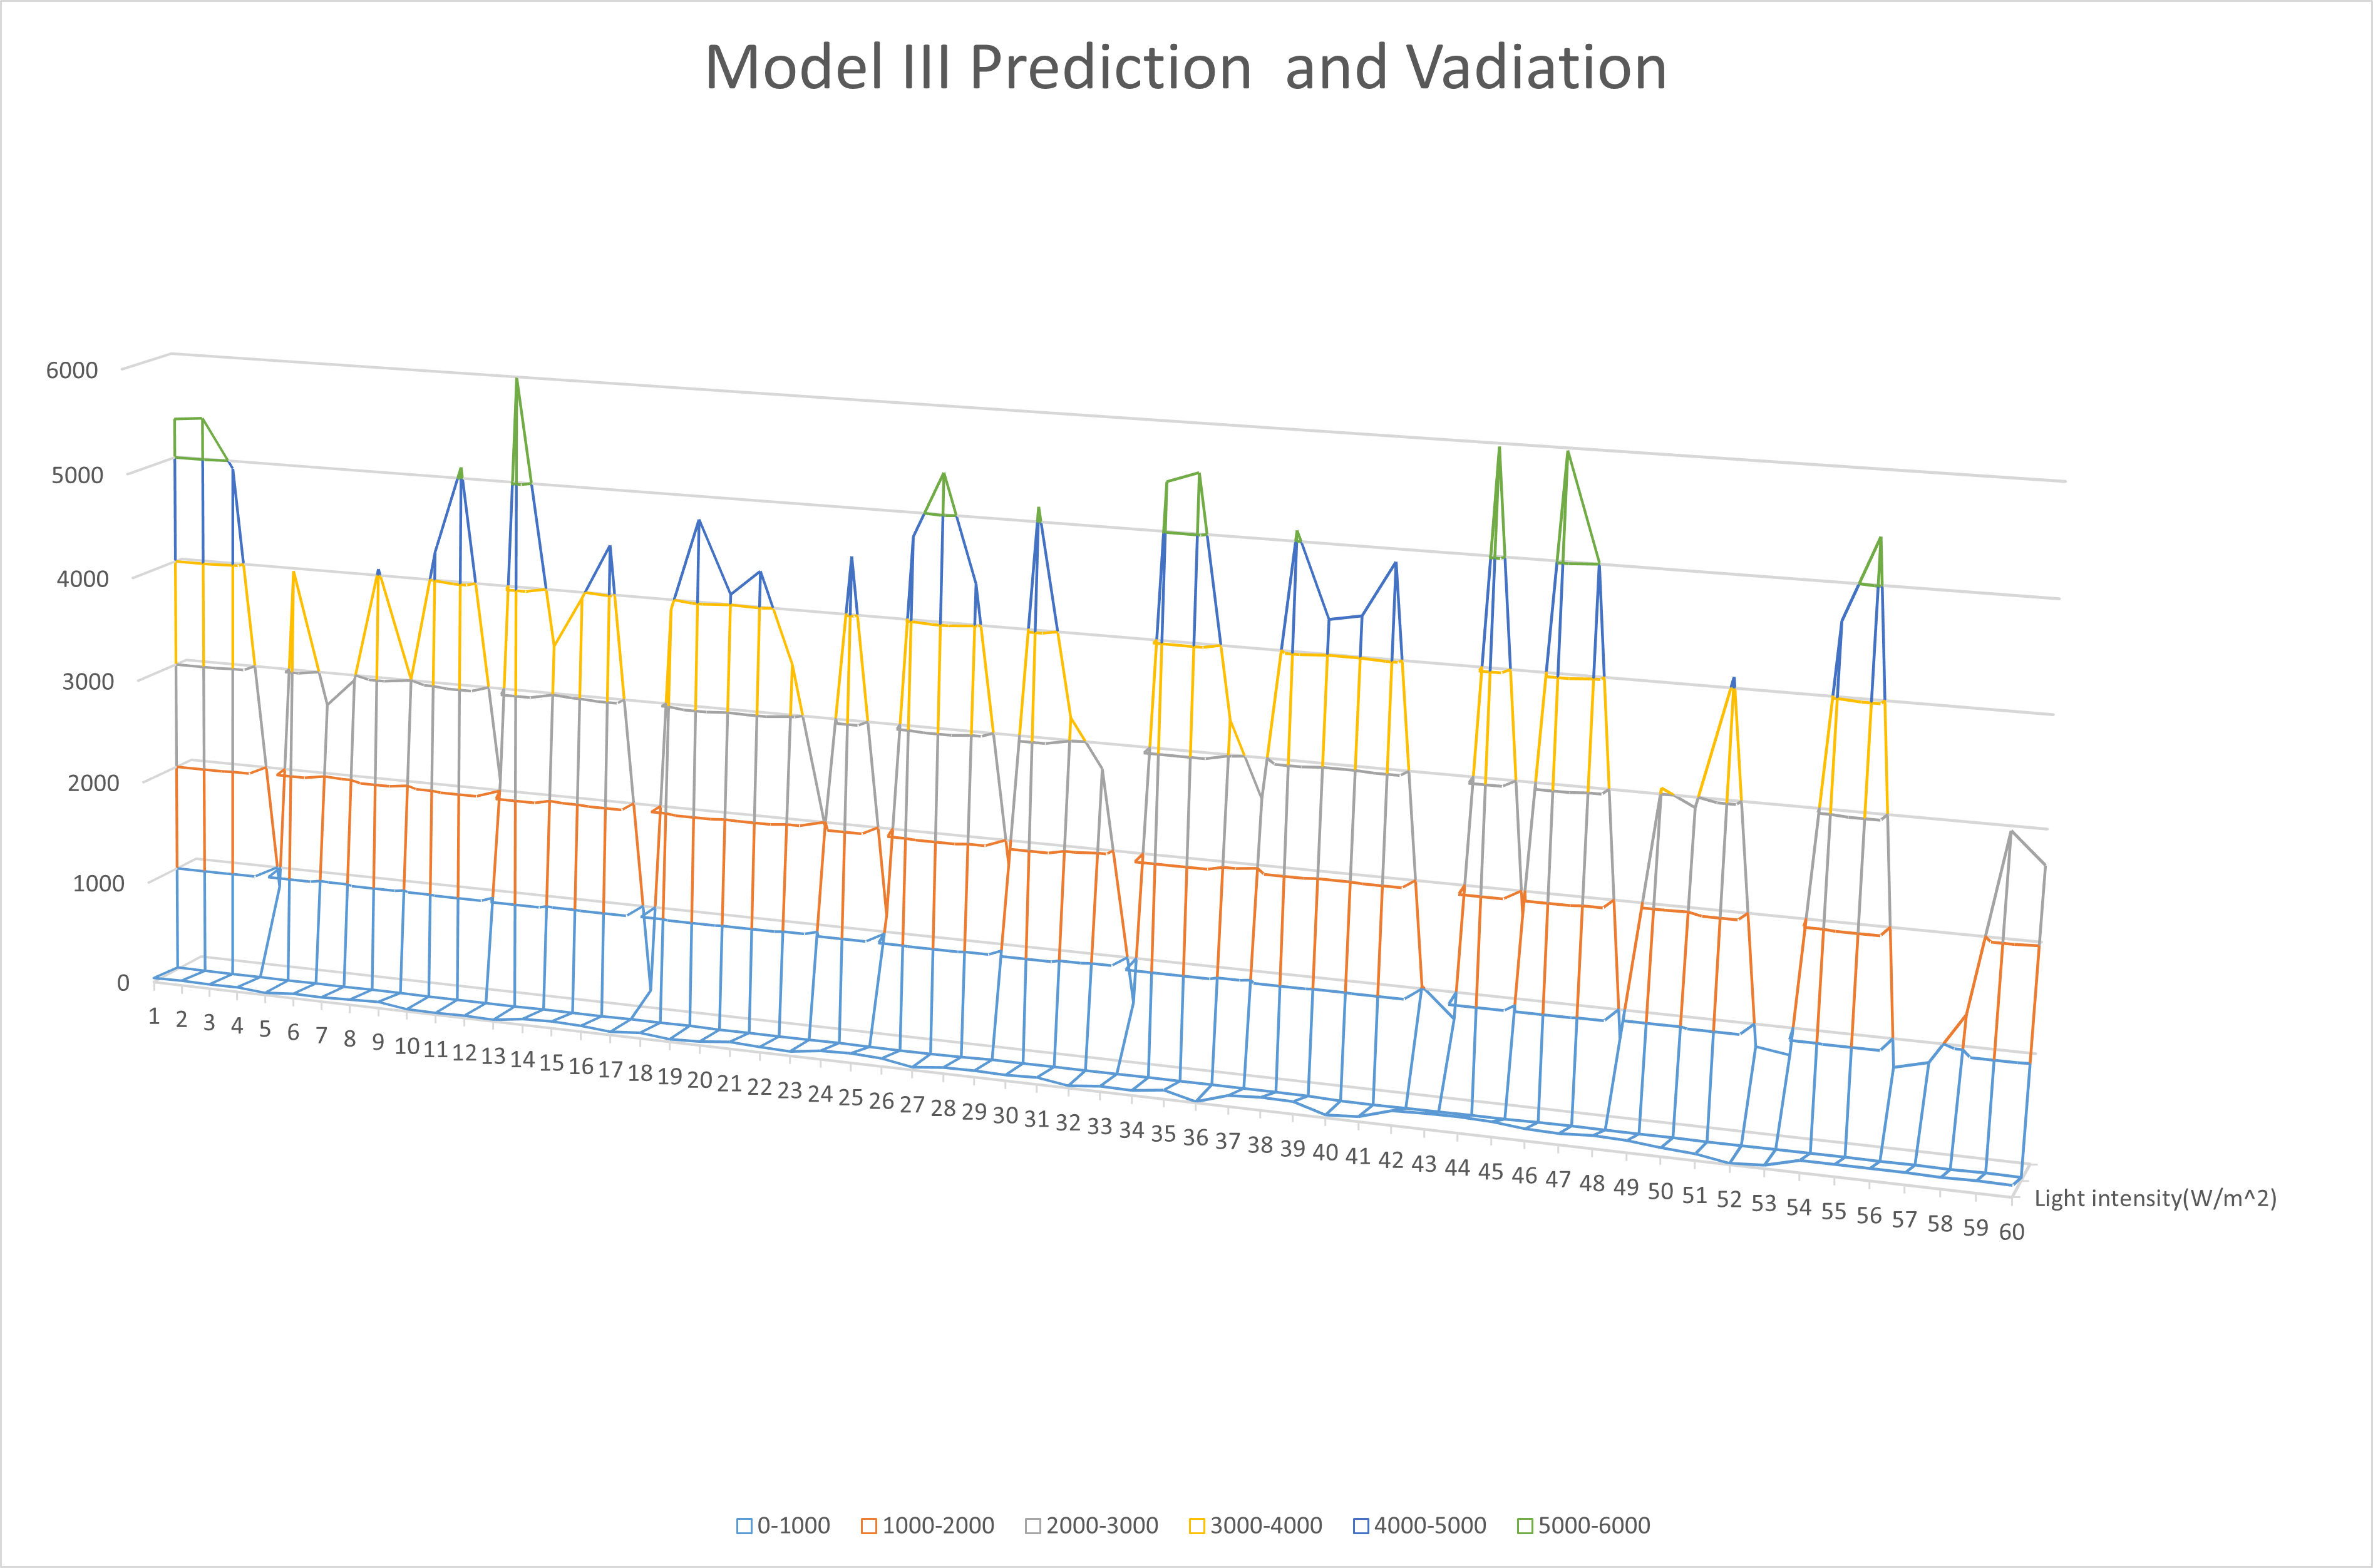
\includegraphics[scale=0.55]{{figure/Model III Prediction and Vadiation.png}}%插入图片的指令
    \caption{Model III Prediction and Vadiation }%标题
    \label{Label}
\end{figure}

We used the relevant data to compare the annual fresh weight and the final output for prediction, and the model output always remained within a certain error range. The stability and extensibility of the model were demonstrated.

%%%%%%%%%%%%%%%%%%%%%%%%%%%%%%%%%%%%%%%%%%%%%%%%%%%%%%%%

\subsection{Application 2: Mechanical ventilation operation model}

Task 5 asked us to consider the case of mechanical ventilation. Since natural ventilation is not stable, the container is mechanically ventilated with fan-driven ventilation. We assume 2 air changes per hour, then 17,520 air changes are required in 1 year time. We combine this with Model III and simply add the energy required for mechanical air changes to the resource consumption of the plant.

According to our survey, centrifugal fans with a backward curved outer cover (backward tilting) have the highest efficiency rating, with a power range P between 10 and 50$kW$ and less than 1kw at static, with an efficiency of $\eta$.
\begin{equation}\label{e1}
	\eta =1.1\ln{P}-2.6+N
\end{equation}
where $N$ means the amount of centrifugal fans.

Considering that our plant plant is a standard 20-foot container, we thought that two fans could be installed to meet the overall ventilation needs. Therefore, the final result of the installation was two centrifugal fans with backward curved outer cover (backward tilting), working twice per hour. Therefore the total energy consumed in the end was$W_{fans}$.
\begin{equation}\label{e1}
	W_{fans} =\frac{(P_{static}\times5+P_{dynamic})}{6}\times24\times365\approx7329.2kW
\end{equation}

After our final analysis, we can conclude that mechanical ventilation requires approximately nearly 7,400 kW of power consumption, which is far less than air conditioning blowing. Although higher than natural ventilation, mechanical ventilation can ensure product quality while enhancing air management and more in line with fire codes. It is a more energy-saving and environmentally friendly ventilation method. It has a very high energy-saving potential.

%%%%%%%%%%%%%%%%%%%%%%%%%%%%%%%%%%%%%%%%%%%%%%%%%%%%%%%%




%下面是之前模板里的常用公式,这里给它们注释掉了
\begin{comment}
\subsection{Equations}

%数学公式:
This is an equation:$$\frac{x}{y}=\frac{\sqrt[3]{x}}{\ln a}$$

This is an equation with number:(Heat Equation)\ref{e1}
\begin{equation}\label{e1}
	c\rho\frac{\partial u}{\partial t}=k\nabla^2u+f
\end{equation}

Matrix:
$$
\left( \begin{matrix}
1&		2&		3&		4\\
a&		b&		c&		d\\
x&		y&		z&		w\\
\alpha&		\beta&		\gamma&		\varphi\\
\end{matrix} \right) 
$$

Integral:

$$
\oint_l{pdx+qdy+rdz}
$$

Some Equation:
\begin{align*}
\cosh x = \frac {1}{2} (e^x + e^{-x}) &= \sum_{n = 0}^{\infty} \frac {x^{2n}}{(2n)!} \\
\sinh x = \frac {1}{2} (e^x - e^{-x}) &= \sum_{n = 0}^{\infty} \frac {x^{2n + 1}}{(2n + 1)!} \\
e^x &= \sum_{n = 0}^{\infty} \frac {x^n}{n!} = \lim_{n\to\infty} \left (1+\frac{x}{n} \right )^n\\
\end{align*}

\subsection{Figures}
This is a figure\ref{fig:comap-logo}:
\begin{figure}[h]
	\centering
	\includegraphics[width=0.7\linewidth]{"figure/comap logo"}
	\caption{Comap logo}
	\label{fig:comap-logo}
\end{figure}

\end{comment}
